\chapter{Problem Description}
\label{chp:relwork}
In this thesis, we introduce ``Credit mining system'', an automatic investment framework on swarm with multidimensional gain. The first phase of the framework was conducted by \citeauthor{2015:creditmining:capota}, mainly to run credit mining system without any restriction or coordination with any client. With credit mining system, locally, a user can gain credit with internally limited bandwidth allocation without any intervention needed. The credit can be in many forms such as share ratio (upload-to-download ratio), uploaded amount, effort based credit, and many other. From higher perspective, credit mining system will help a swarm to keep alive by providing integral pieces to the peer who need it. Although credit mining system will be implemented in Tribler system, it is possible to apply this feature to any system on top of \bt~ network.

In this chapter, several problems that are the main question of this thesis will be elaborated. First we will discuss cooperation and performance problem in peer-to-peer system, specifically \bt. The characteristics and importance of peer-to-peer network and \bt~will be reviewed. Secondly, the issue of \bt~credit and investment will be explained as the main concern of this work. Because Tribler, which we will implement this system into, works in the secure and anonymous environment, some related works on how credit can enforce cooperation in the Tor-like environment will be presented afterwards. Thirdly, we will illustrate how much the bandwidth resource might be consumed by crawling in \bt~ecosystem. Lastly, prior work on credit mining will be reviewed. Further improvements on those work are the core of this thesis.

\section{Peer-to-peer networks}
In this section, we will discuss several aspects of peer-to-peer (P2P) networks. It will start with what and how important P2P currently is. Afterward, we will discuss social challenge that reduces overall performance which also explains peer behavior in P2P. The characteristics of \bt~ applications will be mentioned. Specifically for \bt~community, it is important to know the general classification and what symptom may happen in each community related to performance issue. 

Interaction among user in the Internet community can be expressed in various fashion. Peer-to-peer (P2P) is one of the major interaction existed in the net. This shown in figure \ref{fig:usage}. Many applications and protocols run on top of P2P system, online gaming, computing, and the most popular one, file sharing. \bt~is by far the most popular system used in file-sharing community with its unique \textit{tit-for-tat} mechanism to discourage uncooperative peers \cite{2003:bittorrent:cohen}. 

\begin{figure}[h]
	\centering
	\begin{subfigure}[b]{0.8\textwidth}
		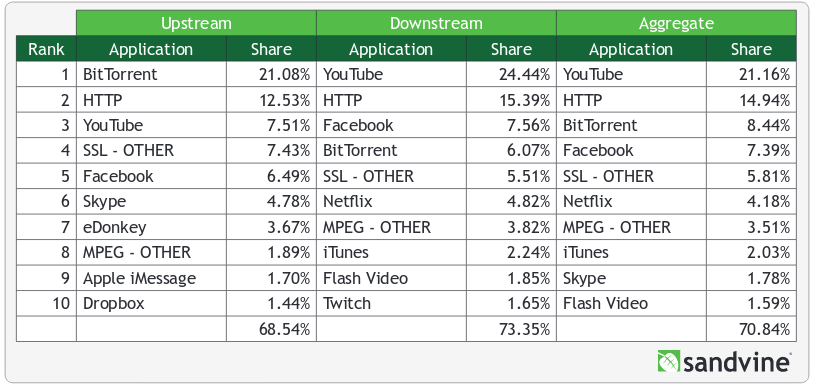
\includegraphics[width=\linewidth]{pics/sandvineeu2015}
		\caption{Sandvine data for 2015 internet usage in Europe}
		\label{fig:usage1}
	\end{subfigure}\\
	\begin{subfigure}[b]{0.8\textwidth}
		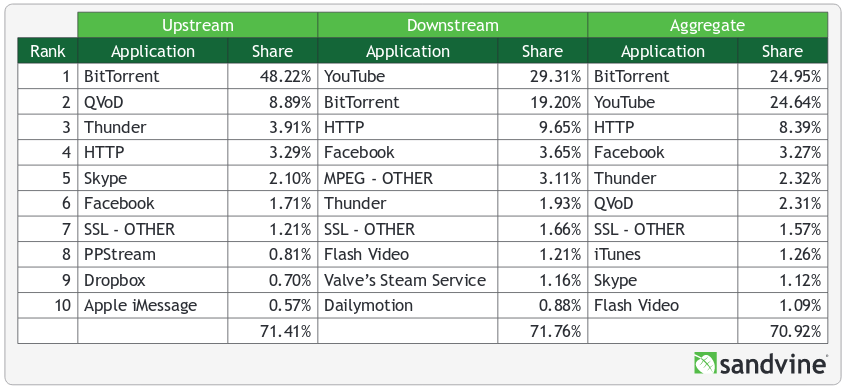
\includegraphics[width=\linewidth]{pics/sandvineasia2015}
		\caption{Sandvine data for 2015 internet usage in Asia Pasific}
		\label{fig:usage2}
	\end{subfigure}%
	\caption{Traffic of the Internet by Sandvine \cite{2015:internettraffic:sandvine}}.
	\label{fig:usage}
\end{figure}

In higher abstraction level, it is common to see P2P system, specifically in \bt, as social networking. Many social challenges, such as incentives mechanism, economic value to survive in the community, reputation identification, and user anonymity, addressed in this kind of network. All of those challenges involves peer behavior whether to help each other for the greater goods, selfishly consume all the resource without giving back, or inconsistently act between these two. It can be interpreted as maximizing their benefits and giving as little as possible. \textit{Freeriding} is the term given to this kind of behavior. It is often to describe this peer as \textit{freeriders}. Based on study by \citeauthor{2000:freeridegnutella:adar}, lots of P2P peers are always show self-interest and rationality, that is, freeriding \cite{2000:freeridegnutella:adar}. In Gnutella case, it even reaches 70\% of its user.  However, \citeauthor{2005:bittorrentcooperation:andrade} showed that \bt~is indeed increased cooperation with only less than 10\% peer is uploading something. In \textit{private community}, this has gone better with higher SLR \cite{2005:bittorrentcooperation:andrade}. Even \citeauthor{2015:freeriderinbtcommunity:das} found that freerider in \bt~ does not deteriorate system performance\cite{2015:freeriderinbtcommunity:das}. All of this fact, however, does not change the fact that P2P users generally are still selfish \cite{2014:userbehaviourprivate:jia}. 

Peer-to-peer networks, not exclusively \bt, has many different applications. Some of them are multimedia streaming, online gaming, and file-transfer. All of those applications has different requirement to ensure user has flawless experience. Multimedia streaming, for example, need to achieve two conditions. First, the start up delay must be small to make sure user do not abandon his intent to stream the files. Secondly, the chunk (or piece) loss must be negligible, or at least low enough to provide good quality\cite{2008:givetogetvod:Mol}. Other application, P2P gaming, require more complex situation. Depend on the type of the game (e.g., FPS), peer latency must be under certain threshold\cite{2010:surveyp2pgame:shen}. It also needs to consider bandwidth demand and high security to prevent cheating between user. The most common P2P application, file transfer, obviously need high throughput by maximizing all the connection a user has.

\subsection{Bittorrent mechanisms}
% tit-for-tat, choking, unchoke, optimistic unchoke
To build \bt~environment, it is essential to know the complete view how \bt~work. In general view, \bt~consists of peers who participated in file-sharing and \textit{tracker}. \textit{Tracker} is responsible for monitors the distribution and progress of the file and peers in the swarm. \textit{Swarm} is a set of peers formed with the same purpose of downloading or uploading certain files represented in \texttt{.torrent} metadata file. Files in a swarm consists of several \textit{chunks} or file pieces. A chunk is exchanged by the peers in a particular \textit{session}. A peer actively participated in many swarms on the uninterrupted time-frame called \textit{session}. 

In \bt, it is desirable to have many peers upload piece of file to the swarm. This way, swarm can be \textit{healthier}, and overall download speed can increase. However, many peers become a \textit{leecher}, which quit the swarm when his download finished. This behavior also called as \textit{Hit and Run} (HnR) \cite{2014:sustainabilitytorrent:chen}. In general, those unwanted behavior normally forbidden in so-called \textit{private communities}. In such a community, the administrator enforces several policy such as \textit{Share Ratio Enforcement} (SRE). SRE define the amount a user need to upload before able to download from the community \cite{2012:economicbt:kash}.

\bt~has distinguished feature to force cooperation of other peers. By peers reciprocation, \bt~ implement \textit{choking algorithm} under its \textit{tit-for-tat} policy. It is basically prioritize peer who provided high upload rates. Choking algorithm is an algorithm to temporarily refuse uploading piece of file to a particular peer. Usually, an uploader has a limited number of unchoked slots. By observing other peers, choking algorithm decides which peer a particular piece will be sent or not sent to. If we unchoke a peer, it means we consider to upload a piece to that peer. For starters, it is usually useful to execute \textit{optimistic unchoking} \cite{2003:bittorrent:cohen}. Optimistic unchoking is an algorithm to unchoke a peer regardless of its activity in a swarm. This gives a peer a chance to increase his upload rate by providing more content. As for downloading, a peer picks \textit{rarest-first} chunk based on the availability in the swarm. This technique make sure that a complete file is distributed in the swarm.

%\todo{expand_:Delivery procedure} -> 

\subsection{Cooperation and performance in \bt}

In a \bt~system, cooperation between peers is crucial to keep a file available in the network. With more user provides the file, the download speed gained for other users will be increased as well. However, this needs user enthusiasm for providing the file regardless of its needs. For both public and private communities, the number of seeders becomes an issue that made a swarm unhealthy \cite{2010:pubpriv:meulpolder, 2014:sustainabilitytorrent:chen}. With freeriders join the swarm, naturally, it will reduce the overall performance. Furthermore, when freeriders become a majority, the swarm is as good as dead \cite{2000:freeridegnutella:adar}. 

\bt~ community can be divided into two categories : \textit{public} and \textit{private}. A community usually served by a \textit{tracker}. Public tracker means everybody can join the swarm served by that tracker. In the other hand, private communities are closed community which can be accessed by passing particular requirement \cite{2010:pubpriv:meulpolder, 2014:sustainabilitytorrent:chen}. \citeauthor{2010:pubpriv:meulpolder} measured that private communities have 3-5 times higher download speed compared to public communities \cite{2010:pubpriv:meulpolder}. This benefit makes joining private community is typically harder compared to public community.

Despite has different performance, both public and private community suffer from a similar issue: ``Poor downloading experience''. It is widely known that public community generally has low SLR which directly affect the swarm performance. In the other hand, private tracker suffers from ``\textit{poor downloading motivation}'' as described by \citeauthor{2014:sustainabilitytorrent:chen}\cite{2014:sustainabilitytorrent:chen} although private community intended to solve low SLR issue. The poor downloading motivation on private tracker affect the sustainability of a swarm. The imbalance of demand and supply will harm new members of private community and gradually degrade the motivation to keep active in the community for another user \cite{2014:sustainabilitytorrent:chen}.

Peer-to-peer file sharing community, especially \bt~ can improve the user downloading experience. It does not give strain to server connection and naturally will download as fast as possible depending on file availability. However, uncooperative peer behavior and low file availability can affect a swarm's health thus reducing download experience. Several kinds of researches already provide solutions to prevent uncooperative peer behavior, all to indirectly push higher downloading throughput on downloader. Most of them focused their work on the incentives for peer or alteration of the currency system itself. Tribler for example, working on a MultiChain \cite{2015:multichain:norberhuis} as a secure and accountable currency in P2P system. \citeauthor{2008:givetogetvod:Mol} published free-riding resilient algorithm for Video on Demand (VoD) in P2P environment\cite{2008:givetogetvod:Mol}. \citeauthor{2015:incentivep2pgame:kang} used game theory as a formulation to incentivize peer in order to prevent free-riding behaviour\cite{2015:incentivep2pgame:kang}. They also considered mobile P2P network which only capable of low complexity mechanism. In their work, peers are awarded with different credit depend on connection type and content.
% problem: p2p social community is good if all peer is considerable, otherwise, it sucks.bittorrent pattern flashcrowd : many S/L, only at the beginning.  deteriorate afterwards. User rewarded for providing old content?
% probably not
% reputation, credit

\section{The confusion in \bt~credit investment}
In peer-to-peer system, specifically in \bt~protocol, \textit{incentive mechanism} is introduced to tackle freeriding problem \cite{2003:bittorrent:cohen}. With limited resource possessed by each peer, there is a price that need to be paid on accessing resource. The whole collection of transaction created incentive system which should be defined in order to extract user goodness in computational way.

In economic terminology, it is necessary to specify a value of the resource that can lead to the ``wealth'' of a user. In \bt~system ``credit'' can be defined in various object. For specific, private community such as DIME\footnote{\url{www.dimeadozen.org}}, \citeauthor{2012:economicbt:kash}  defined credit as \texttt{4 x upload - download} in bytes, accumulated for all the torrent served in that community \cite{2012:economicbt:kash}. \citeauthor{2015:creditmining:capota} assume the credit on his work as the difference between uploaded and downloaded bytes. \citeauthor{2014:sustainabilitytorrent:chen} mentioned another form of credit that can be earned depend on the activity, for example, seeding more torrents, seeding longer and old torrent, and seeding torrent that consumes large disk space\cite{2014:sustainabilitytorrent:chen}. In \bt, incentive system is enforced by its choking algorithm. It prefers to give the resource to the one who has the highest credit, in this case, the upload rate. In general file-sharing peer-to-peer application, user will receive credit when they upload data to others.

With credit as a token of incentive, user can ``spend'' the credit to get service from someone else. In many communities, this means that user can download more files. It is also possible that this credit may be spent to get other facilities in the community such as right to access specific content, get higher download speed, and receive social acknowledgement. Naturally, having many credit as user disposal may be advantageous \cite{2014:sustainabilitytorrent:chen}. At the point user aware of this achievement, he may want to \textit{invest} his already owned credit to get more credit.

Although high credit for user is desirable, one must be aware the effect of overwhelming credit on few users is bad for the community. Therefore, it is important to balance credit mining and community overall performance. \citeauthor{2015:sustainabilitypt:vinko} showed that both of them have conflicting interest. High few individual performance can lead to lower overall community performance \cite{2015:sustainabilitypt:vinko}. Moreover, \citeauthor{2013:survivepriv:jia} also mentioned that oversupply swarm because of overwhelming seeders may result in lower bandwidth allocation for other users \cite{2013:survivepriv:jia}. Not to mention undersupply problem that common in public community which gives very poor performance.

We define the activity of downloading with the expectation of obtaining credit to use later on as \textit{investment}. The act of seeding to help to increase the community performance graciously is called \textit{donating}. A user can \textit{prospect} which community he will invest or donate regardless of his own resource. Not all the swarm need to be seeded as we shown the drawbacks of oversupply. The prospecting and identifying swarm that needs to be seeded based on the seeder's intention (whether to invest or donate) is important. By providing proper prospecting function, users could help each other to improve the swarm quality. In good investing algorithm, users can make better use of its resource to gain credits when prospecting a swarm. 

To the best of our knowledge, there are very few works addressed credit investment in \bt. \citeauthor{2013:survivepriv:jia} mentioned how inefficient the practice of seeding for a long time to get credits. Ironically, the long time seeding is commonly practiced as it is the most trivial way to maintain credits \cite{2013:survivepriv:jia}. Three prior work has been done by \citeauthor{2015:creditmining:capota} \cite{2015:creditmining:capota, 2013:investmentcm:capota, 2014:bwmarket:capota}. This will be discussed in section \ref{section:cmprior}. 

\subsection{Secure Currency}
In this section, we will discuss how the credit system may work in the secure environment. The most common secure environment applicable in a peer-to-peer network is depicted by \textit{onion routing}. With onion routing, the connection or transaction from one peer must be relayed via another peer before reaching their destination. This requires alteration of the incentive mechanism. Some of the related incentive mechanism are MultiChain \cite{2015:multichain:norberhuis}, LIRA \cite{2013:lira:jansen}, and TorCoin \cite{2014:torcoin:ghosh}. Although LIRA and TorCoin not used in \bt~ecosystem, it still gives insight how the incentive mechanism work with the onion routing used in Tribler.

Tribler used to have secure reputation system called BarterCast4 \cite{2009:bartercast:meulpolder}. Reputation system in a sense, can be used as an incentive mechanism. A user, may receive high reputation if he provide quality content, and may lose reputation if he cheat in the system. Although BarterCast is fully decentralized, the system is vulnerable from attacks. BarterCast4 has no security measure to prevent tampering records. As \citeauthor{2015:multichain:norberhuis} pointed, BarterCast uses self-reported reputation as its base. It is possible for someone change his reputation arbitrarily, then use it to get higher priority in data transaction. MultiChain, introduced in 2015, addressed to solve this issue and will replace BarterCast as the currency in the Tribler community \cite{2015:multichain:norberhuis}. 

MultiChain is a secure reputation system which contains interaction history between corresponded peers in a distributed environment \cite{2015:multichain:norberhuis}. MultiChain is inspired by the Block chain technology implemented in cryptocurrency such as Bitcoin. The difference is, if Bitcoin represents computation, MultiChain represents bandwidth used. In blockchain, multiple transactions are combined into a single block. A single block has a pointer to the previous block. If a peer \texttt{A} upload a file to peer \texttt{B}, \texttt{A} may want to increase its reputation by write it to the MultiChain. This transaction is transcribed into one MultiChain block. This block is protected by confirmed signature from both parties, \texttt{A} and \texttt{B}. The protected block can be easily verified by other peer. Note that MultiChain only reputation system. Incentive mechanism is still needed to assign proper reward and punishment fo honest peer and freeriders.

In a secure network with onion routing, one who relay the network at the cost of its bandwidth need to be incentivized as well. LIRA \cite{2013:lira:jansen} offers lightweight incentive system for user who contribute for the Tor network. It is based on the probability on getting lottery. The lottery itself is a priority on the Tor network which will improve the client performance. However, as LIRA is based on centralized bank in Tor's network, it still induced scalability problem. TorCoin \cite{2014:torcoin:ghosh} is another work covering this issue. Similar with MultiChain, TorCoin proof-of-work is its bandwidth embedded in the blockchain mechanism. This work also preserves anonymity, enforces accounting mechanism, and deploys in fully distributed manner. The main problem of TorCoin is that it requires extra specific protocol in Tor that not yet implementable called TorPath. TorPath is a protocol that assign a secure circuit to each client, monitor the route, and generate TorCoin as a proof or relaying or providing bandwidth to other user. In overview, there are three steps of TorPath. First is TorPath forms a group of users to interconnect each other. After that it shuffles and assign the circuit. At this point, Tor circuit is established and then each of the client can route with this established circuit. TorCoin can be mined by user via this TorPath.

\section{Optimizing resource}
To gain credit, seeding is necessary. However, users are forced to seed for excessively long time to maintain adequate credit \cite{2013:survivepriv:jia}. \citeauthor{2013:survivepriv:jia} also stated that this activity is commonly practiced although it is not productive. By seeding unproductively, user wastes his resources, such as bandwidth, storage capacity, and computer power.

In larger scale, if we meant to seed a lot of torrents, for example, a million, the bottleneck occurred will be more fundamental. \citeauthor{2012:milliontorrent:arvid} shows an example how costly the \textit{announce} request accompanied by \textit{response} payload can be. Seeding 1 million torrent with announce once per every hour, which is half of the default interval, need 130 kB//s upload and 75 kB//s download bandwidth constantly \cite{2012:milliontorrent:arvid}. This value is significant for most of common Internet connection.

Most researches have measured \bt~ by crawling its community pages \cite{2013:survivepriv:jia, 2005:bittorrentcooperation:andrade, 2014:userbehaviourprivate:jia, 2010:pubpriv:meulpolder, 2014:sustainabilitytorrent:chen, 2012:economicbt:kash, 2013:investmentcm:capota, 2009:demandsupplyres:andrade, 2011:interswarm:capota}. This way, they can get the data summarized by the pages. Some researches contact the tracker regularly or using its dump logs \cite{2011:yoshida:crawlbtnet, 2005:bittorrentcooperation:andrade,  2015:freeriderinbtcommunity:das, 2011:interswarm:capota}. Most of the research using logs as its dataset only use single tracker to monitor a particular torrent. Few of the research use instrumented client or directly observe the \bt~environment by understanding peer behavior \cite{2010:pubpriv:meulpolder, 2013:swarmevolution:su}. A work conducted by \citeauthor{2010:btworld:wojciechowski} discussed several method of \bt~measurement. The methods shown in table \ref{tbl:btmeasuremethod}.

\begin{table}[ht]
	\centering
	\caption{\bt~measurement techniques \cite{2010:btworld:wojciechowski}}
	\label{tbl:btmeasuremethod}
	\begin{tabular}{|l|l|l|}
		\hline
		\rowcolor[HTML]{C0C0C0} 
		\multicolumn{1}{|c|}{\cellcolor[HTML]{C0C0C0}\textbf{Level}} & \multicolumn{1}{c|}{\cellcolor[HTML]{C0C0C0}\textbf{Advantage}} & \multicolumn{1}{c|}{\cellcolor[HTML]{C0C0C0}\textbf{Disadvantage}} \\ \hline
		Internet & Excellent coverage & ISP collaboration \\ \hline
		Community & Implementation & Peer details \\ \hline
		Swarm & Details & Context \\ \hline
		Peer & Details & Scalability \\ \hline
	\end{tabular}
\end{table}

In the following section, we will focus on the measurement technique with peer discovery. With the trackless \bt evolved in early 2008 by DHT protocol \cite{2008:dht:loewenstern}, monitoring trackers may result in inaccurate result. Moreover, the credit mining mechanism heavily rely on real-time data which can not be obtained from querying the community pages.

% peer discovery DHT, PEX, LSD
\subsection{Peer Discovery}
One of the integral part in \bt~protocol is peer discovery. With numerous known peers, the algorithm will have more option on which peer to unchoke. State of the swarm itself often represented by the peer belong to that swarm. As mentioned before, it is relatively costly just to discover new peers if there are a lot of swarms monitored. 

In \bt, there are four methods to discover new or update peer. Those are using centralized trackers, distributed hash table (DHT), peer exchange (PEX), and local service discovery (LSD). The methods will be described below.

\subsubsection{Tracker Peer Announce}
In original design of \bt, it uses tracker to allow peer discover each other \cite{2003:bittorrent:cohen}. Tracker tends to use random and limited list of peers. Peer contact tracker periodically to expand their peer dictionary. This act of requesting peer to tracker is called \textit{announce}.	Usually, most tracker has a policy about recommended interval when to recontact for getting new peers. Violate this policy can result a particular peer blocked.	
	
\subsubsection{Distributed Hash Table (DHT)}
Originally, peer needs to contact tracker to fetch new peer address and file information. This makes \bt~very dependent on centralized system which vulnerable to single point of failure. In 2008, Distributed Hash Table (DHT) was proposed \cite{2008:dht:loewenstern}. Towards a ``trackerless'' \bt~system, DHT allows each peer to become a tracker. DHT stores peer contact information with defined key-space as ``node ID''. Each peer stored other peer's node ID and its address in their own routing table. A ``distance'' is measured on two node ID to define how close those two. ``Distance'' also can be measured between infohash of a torrent and node ID.
	
To enrich its peer dictionary, a node can compare a torrent's infohash and node ID in its routing table. If the distance under the threshold, it contacts that node to ask the information of the swarm, which includes the peer list. If contacted node do not know this torrent, it will respond with another node in its table which closest to the provided infohash. 
%\todo{expand_:DHT performance?}

\subsubsection{Peer Exchange (PEX)}
To increase the chance of getting higher downloading speed, having up to date peer is desired. This can be achieved by contacting tracker or using DHT. Reducing the interval of contacting tracker can result in getting a number of updated peer sooner, however, it will put a burden on the tracker itself. Peer Exchange (PEX )\cite{2015:PEX:the8472} is proposed to tackle this problem. PEX used list of peers that bootstrapped from another mechanism. This mechanism allows contacting known peer directly to get and give up-to-date information on swarm. Theoretically, it can keep this swarm together if trackers are down. Specification mentioned in \cite{2015:PEX:the8472} stated a restriction such as number of request per minute and number of peer added or removed in a PEX message.
	
\subsubsection{Local Service Directory (LSD)}
To increase the performance when downloading from a swarm, it is preferable to get the file from local network if available. Local service directory (LSD) permit this by discover peers that are in the same local network. The transfer rate is much higher compared to other type of peers. In short, LSD uses multicast-like mechanism which broadcast infohash of a torrent.
%\\
%Anonymous Relaying performance in Tribler \cite{2015:onionroutetribler:stokkink}\\
%Significant portion when seeding million torrents \cite{2012:milliontorrent:arvid}
%
%check swarm scrape -> multiple research -> based on dump logs

% piece population study -> http://ieeexplore.ieee.org/document/4410992/?arnumber=4410992
% related : Legout's work

% characteristics : http://www.sciencedirect.com/science/article/pii/S1389128610003622

\section{Credit Mining Framework}
\label{section:cmprior}
Preliminary work on credit mining has been done by \citeauthor{2015:creditmining:capota} \cite{2015:creditmining:capota, 2013:investmentcm:capota, 2014:bwmarket:capota}. At the first phase, they implement complex method with speculative download to assess the swarms\cite{2013:investmentcm:capota}. Extending this work, they introduced \textit{helper} peer to seed low capacity swarm using libtorrent \textit{share mode}\cite{2014:bwmarket:capota}. Recently, they moved into multiple swarm approach and using public community as their research object. With swarm selection policy, they observed whether helper peer can generate high credit with less downloading\cite{2015:creditmining:capota}.

\begin{figure}[ht]
	\centering
	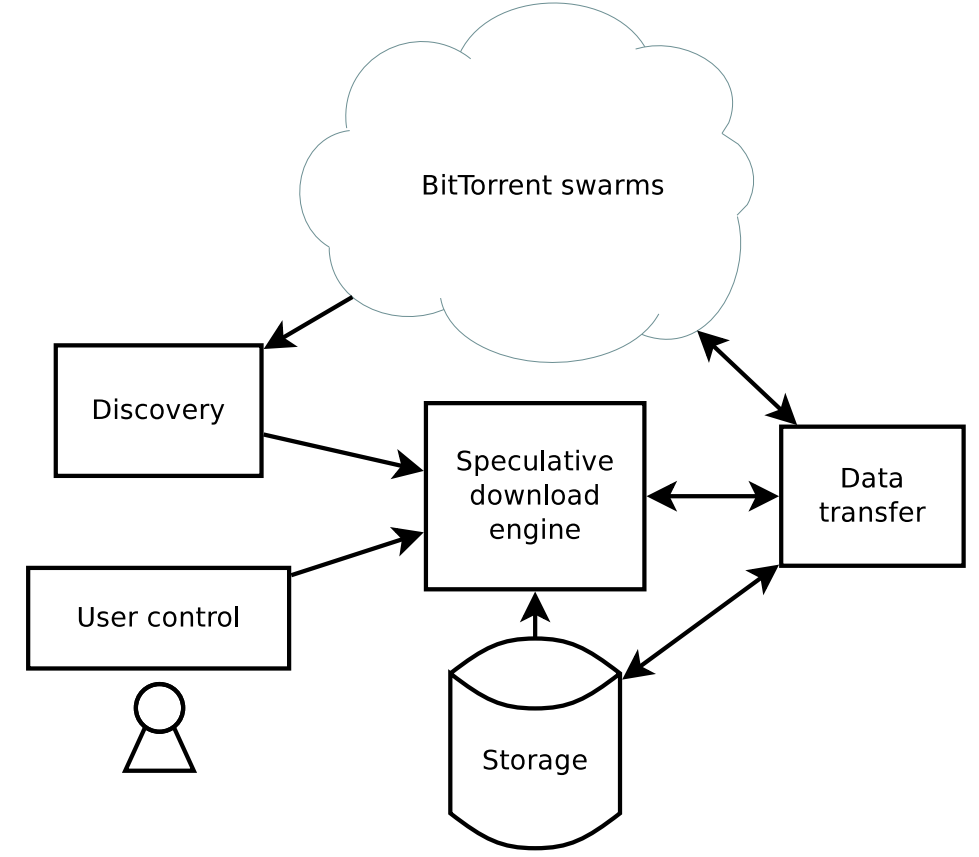
\includegraphics[width=0.7\textwidth]{pics/SDE2013.png}
	\caption{Speculative download mechanism \cite{2013:investmentcm:capota}}.
	\label{fig:sde13}
\end{figure}

In \citeyear{2013:investmentcm:capota}, \citeauthor{2013:investmentcm:capota} introduced bandwidth investing in \bt~private communities. He applied speculative download (as shown in figure \ref{fig:sde13}) on prospected swarm. This research used activity data crawled from Bitsoup\footnote{\url{https://www.bitsoup.me}} to evaluate their system. Every swarm is analyzed whether it will keep the swarm in \textit{cache} or discard it. Swarm is scored by predicting future upload speed defined in multiple regression model\cite{2013:investmentcm:capota}. One of the findings is that this algorithm depends on the size of the evaluated swarm. The more swarm need to be assessed, there is less chance the algorithm will find suitable cache to replace. This also shows the high costs and complexity of \textit{multivariate adaptive regression splines} (MARS) implemented in this system.

A year after, in \citeyear{2014:bwmarket:capota}, a research to align supply and demand in \bt~network is conducted. The idea is each peer monitor their swarms to detect whether there will be potential undersupply. If such a condition is found, one will broadcast \textit{help request} to specialized peers in order to seed this swarm. Specialized peers, called \textit{helpers}, tries to download as little as possible while upload as much as possible using \textit{libtorrent} share mode. They implement multiple helper and observe its effect to swarm with actual downloading on the other side. Their experiment result shows that using share mode in closed environment will increase download performance if the bandwidth is underutilized \cite{2014:bwmarket:capota} by shifting the bottleneck in the swarm. Moreover, \textit{libtorrent} share mode is also proven to be able to detect whether a swarm has enough capacity or not. This research also discussed flash crowd scenario. In this scenario, the existence of helper peer can lead leecher peer to reach higher download speed, especially in the early time of scenario. 

The most recent work was conducted in \citeyear{2015:creditmining:capota}\cite{2015:creditmining:capota}. \citeauthor{2015:creditmining:capota} incorporated his previous work into Credit Mining System implemented in Tribler. credit mining system able to monitor multiple swarm in one moment, and then decide which swarm this system will donate its bandwidth to. It uses simpler policy on choosing swarm compared to multivariate regression model in \cite{2013:investmentcm:capota}. As policy input, credit mining system uses torrent parameters such as seeder and leecher number obtained from tracker/DHT, creation date, length, and many others. The overview of mining process is shown in figure \ref{fig:cm15}. The experiment was conducted in live fashion on RSS \textit{etree.org}\footnote{\url{http://bt.etree.org/rss/bt\_etree\_org.rdf}} public community. They observed \textit{net upload gain} which defined as difference of uploaded bytes and downloaded bytes. Proposed policy and framework resulted in positive effect to the community.

\begin{figure}[ht]
	\centering
	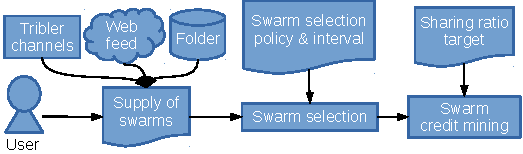
\includegraphics[width=0.8\textwidth]{pics/creditmining2015.pdf}
	\caption{The overview of credit mining process \cite{2015:creditmining:capota}}.
	\label{fig:cm15}
\end{figure}

\section{Research Objective}
The main objective of this thesis is to implement and extend credit mining system in Tribler. There was prior work on credit mining with basic capabilities described in \cite{2015:creditmining:capota}. This thesis also based on prior work reported in  \cite{2013:investmentcm:capota} and  \cite{2014:bwmarket:capota}. 

The next step of credit mining system is to fully integrate it with Tribler. Currently this system is in broken state with its incompatibility with Tribler. There is minimal use of Tribler feature such as anonymity and social feature. The prior work on credit mining system will be elaborated in detail in section \ref{section:cmprior}. The implementation will consider user activity and its experiment will be conducted in production level. With this in mind, in this thesis we tried to answer the following research question : 

\noindent{
	\\
	\textit{How do we fully incorporate credit mining system in Tribler?}
	\\}

In order to answer the question, we formulate technical challenge that need to be solved. The challenges include engineering and performance evaluation aspect. The questions are the following : 

\begin{enumerate}
	\item \textit{What is the effect of mining in background for end-user?}
	\\ In the prior work, a \textit{helper} system was exist. However, either it was limited to one role per peer or all the peer in the swarm have single role. While this approach is reasonable, it is unlikely that a peer will stick to one behavior. A peer may download normally from a swarm in one time, while decide to graciously help another swarm in other time.
	
	\item \textit{How do we take advantage of unused bandwidth in Tribler client in non-disruptive manner?}
	\\ Downloading from \bt~network may or may not consume all of the peer bandwidth. If a user download from many swarm simultaneously, he has higher chance of utilizing his bandwidth to the most. Otherwise, the bandwidth is wasted. In the previous work, it is assumed that credit mining system will consume all the bandwidth. Naturally, it took part of the bandwidth and reduced user's experience. The system address this issue by proposing activity-aware mechanism. The purpose is to get the most out of the bandwidth without disturb user of his own activity.
	
	%	\item \textit{How is the performance of continuous-automatic\todo{perhaps +anonymous}~ mining?} 
	%		\\ Several credit mining performance have been discussed in \cite{2015:creditmining:capota} and \cite{2014:bwmarket:capota}. With alteration of the mechanism, it is natural to reevaluate the system. It is also important to study, if any, the drawbacks occurred with the integration.
	\item \textit{How to prospect swarm and what is good investment?}
	\\ The idea of credit mining system is to help undercapacity swarm while at the same time to get credit for uploading data. Finding which swarm that might have high return is called \textit{prospecting}. \textit{Investing}, specifically, consider prospecting in limited resources as additional requirement. Resource can be in several forms such as bandwidth, memory, or storage. Although the term ``good'' may be relative, we intend to show the efficiency of credit mining from different aspect.
	
	\item \textit{What is the effect of credit mining system in live production environment?}
	\\ While previous question address local effect to user, this questions whether automatically mining or donating bandwidth can lead to increasing swarm capacity. Many characteristic of swarm start form low seeder, practically dead swarm, and new published swarm will be considered. Does credit mining really has positive impact on the swarm?
	
	\item \textit{What properties in Tribler that credit mining system can use to improve the experience and how?}
	\\ Tribler consists of multiple modules. In section \ref{section:tribler} some of the features will be discussed. To fully integrate credit mining system with Tribler, it is intriguing to understand what Tribler client can offer to improve user experience within this system. Specifically, we will focus on the anonymity and Tribler torrent collection within its channel.
\end{enumerate}

%
%\subsection{MultiChain}
